\documentclass[aspectratio=169, 10pt]{beamer}
\usetheme[progressbar=frametitle]{metropolis}
\usefonttheme{serif}

\usepackage{lmodern}
\usepackage{graphicx}
\usepackage{amssymb}
\usepackage{amsmath}
\usepackage{latexsym}
\usepackage{xcolor}
\usepackage{hyperref}
\usepackage{adjustbox}
\usepackage{mathtools}
\usepackage{multicol}

\usepackage{tikz}
\usetikzlibrary{arrows, arrows.meta, positioning, shapes.geometric, calc, decorations.pathreplacing, fit}
\usetikzlibrary{backgrounds, angles, quotes}

\input{colors}

% ---- accent colors (from colors.tex palette) ----
\colorlet{CCGAred}{red}
\colorlet{CCGAblue}{blue}
\colorlet{CCGAgreen}{green}

% ---- math macros (CCGA notation) ----
\newcommand{\eo}{\mathbf{e}_o}
\newcommand{\einff}{\mathbf{e}_\infty}
\newcommand{\eob}{\bar{\mathbf{e}}_o}
\newcommand{\einfb}{\bar{\mathbf{e}}_\infty}
\newcommand{\eoi}[1]{\mathbf{e}_{o_{#1}}}
\newcommand{\einfi}[1]{\mathbf{e}_{\infty_{#1}}}
\newcommand{\Iod}{I_o^{\triangleright}}
\newcommand{\Iinfd}{I_\infty^{\triangleright}}
\newcommand{\Io}{I_o}
\newcommand{\Iinf}{I_\infty}
\newcommand{\Ieps}{I_\varepsilon}
\newcommand{\wed}{\wedge}
\newcommand{\meet}{\vee}
\newcommand{\dotp}{\cdot}
\newcommand{\vinf}{v_\infty}
\newcommand{\R}[1]{\mathbb{R}^{#1}}
\newcommand{\pca}{p_c}

%%%%%%%%%%%%%%%%%%%%%%%%%%%%%%%%%%%%%%%%%%%%%%%%%%%%%%%%%%%%%%%%%%%%
\title{Conic Conformal Geometric Algebra\\[2pt]\large Completing the Object Algebra}
\institute[LIGM \& LAMA]{LIGM, Universit\'e Gustave Eiffel \quad LAMA, Universit\'e Savoie Mont-Blanc, CNRS}
\author[Harquin et al.]{\small \textbf{Enzo Harquin}$^1$, St\'ephane Breuils$^2$, Venceslas Biri$^1$, Vincent Nozick$^1$}
\date{\alert{ENGAGE 2026 --- London}}
%%%%%%%%%%%%%%%%%%%%%%%%%%%%%%%%%%%%%%%%%%%%%%%%%%%%%%%%%%%%%%%%%%%%

\begin{document}

% ============================================================
% A. TITLE & MOTIVATION
% ============================================================
\begin{frame}
  \titlepage
\end{frame}

\begin{frame}[t]{Motivation: from circles to all conics}
  \setlength{\columnsep}{20pt}
  \begin{columns}[T]
    \column{0.54\textwidth}
      \textbf{Conformal GA (CGA)} models \alert{round} objects natively:
      points, lines, \alert{circles}, spheres --- one isotropic radius.

      \vspace{0.5cm}
      But an \alert{ellipse}, \alert{hyperbola}, \alert{parabola}, or a
      \alert{tilted} conic is \emph{not} round. Classically they need ad-hoc
      $3{\times}3$ matrices, handled \emph{outside} the algebra.

      \vspace{0.5cm}
      \textbf{Goal.} A single geometric algebra in which \alert{every conic} is
      one object --- built from points by $\wed$, intersected by $\meet$,
      with a clean dual.

    \column{0.46\textwidth}
      \centering
      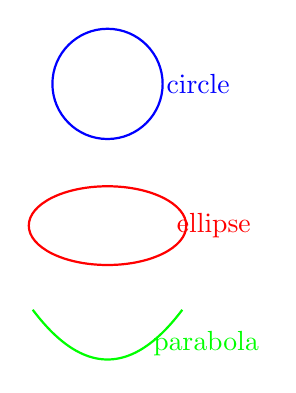
\begin{tikzpicture}[scale=1.0]
        \draw[CCGAblue, thick] (0,0.9) circle (0.7);
        \node[CCGAblue] at (1.15,0.9) {circle};
        \draw[CCGAred, thick] (0,-0.9) ellipse (1.0 and 0.5);
        \node[CCGAred] at (1.35,-0.9) {ellipse};
        \draw[CCGAgreen, thick, domain=-0.95:0.95, samples=60, variable=\t]
          plot ({\t},{-2.6+0.7*\t*\t});
        \node[CCGAgreen] at (1.25,-2.4) {parabola};
      \end{tikzpicture}\\[0.2cm]
      {\small CGA reaches only the top one.}
  \end{columns}
\end{frame}

% ============================================================
% B. CGA REMINDER (single slide)
% ============================================================
\section{From CGA to CCGA}

\begin{frame}[t]{Conformal GA in one slide}
  \setlength{\columnsep}{18pt}
  \begin{columns}[T]
    \column{0.6\textwidth}
      Conformal model $\R{4,1}$, \alert{null basis} $\eo,\einff$:
      \[
        \eo^2=\einff^2=0,\qquad \eo\dotp\einff=-1 .
      \]
      A point $(x,y)$ lifts to a \alert{null vector}; the metric is Euclidean distance:
      \[
        p = \eo + x\,\mathbf{e}_1 + y\,\mathbf{e}_2 + \tfrac12(x^2+y^2)\,\einff,
        \qquad p^2=0,
      \]
      \[
        p\dotp q = -\tfrac12\,\mathrm{dist}(p,q)^2 .
      \]
      A circle / sphere is the \alert{IPNS vector}
      \[
        s = \pca - \tfrac{r^2}{2}\,\einff,\qquad s^2=r^2 .
      \]

    \column{0.4\textwidth}
      \begin{alertblock}{The ceiling}
        A \alert{single isotropic radius} $-\tfrac{r^2}2\einff$ $\Rightarrow$ the locus is
        always a \alert{circle}.
      \end{alertblock}
      A general conic
      \[
        Ax^2{+}By^2{+}Cxy{+}Dx{+}Ey{+}F=0
      \]
      has \alert{six} coefficients --- the \alert{degree-2 Veronese} of $(x,y)$.
      Embed \emph{that}.
  \end{columns}
\end{frame}

% ============================================================
% C. CCGA ALGEBRA
% ============================================================
\section{CCGA: the algebra}

\begin{frame}[t]{The algebra $\R{5,3}$}
  Three conformal copies: signature $\R{5,3,0}$ (\alert{non-degenerate}).
  \[
    \underbrace{\mathbf{e}_1,\mathbf{e}_2}_{+},\qquad
    \underbrace{\mathbf{e}_{+1},\mathbf{e}_{+2},\mathbf{e}_{+3}}_{+},\qquad
    \underbrace{\mathbf{e}_{-1},\mathbf{e}_{-2},\mathbf{e}_{-3}}_{-} .
  \]
  \alert{Null basis} ($i=1,2,3$):
  \[
    \eoi{i}=\mathbf{e}_{+i}+\mathbf{e}_{-i},\qquad
    \einfi{i}=\tfrac12(\mathbf{e}_{-i}-\mathbf{e}_{+i}),
  \]
  \[
    \eoi{i}^2=\einfi{i}^2=0,\quad \eoi{i}\dotp\einfi{i}=-1,\quad
    \mathbf{e}_1\dotp\mathbf{e}_1=\mathbf{e}_2\dotp\mathbf{e}_2=1 .
  \]
  \vspace{0.2cm}
  \begin{exampleblock}{Why $\R{5,3}$ and not a degenerate metric}
    Non-degenerate $\Rightarrow$ the pseudoscalar $I$ is invertible $\Rightarrow$
    \alert{dual, meet and join are all clean} (unlike PGA).
  \end{exampleblock}
\end{frame}

\begin{frame}[t]{Special blades and the two gauge bivectors}
  Two mutually orthogonal conformal pairs --- a Euclidean one and a differential one:
  \[
    \eo=\eoi1+\eoi2,\quad \einff=\tfrac12(\einfi1+\einfi2),\qquad
    \eob=\eoi1-\eoi2,\quad \einfb=\tfrac12(\einfi1-\einfi2),
  \]
  \[
    \eo\dotp\einff=-1,\qquad \eob\dotp\einfb=-1,\qquad \{\eo,\einff\}\perp\{\eob,\einfb\}.
  \]
  The two \alert{gauge bivectors} that organise everything:
  \[
    \boxed{\;\Iod=\eob\wed\eoi3\;}\ \text{(origin gauge)}
    \qquad\qquad
    \boxed{\;\Iinfd=(\einfi1-\einfi2)\wed\einfi3\;}\ \text{(infinity gauge)} .
  \]
  Top blades $\Io=\eoi1\wed\eoi2\wed\eoi3$, $\Iinf=\einfi1\wed\einfi2\wed\einfi3$,
  $\Ieps=\mathbf{e}_1\wed\mathbf{e}_2$, pseudoscalar
  $I=\Ieps\wed\Iinf\wed\Io$ with $I^2=-1$.
  \vspace{0.15cm}

  \textcolor{gray}{Dual $A^\star=A\,I^{-1}$, undual $A\,I$; join $A\wed B$; meet $A\meet B=(A^\star\wed B^\star)^\star$.}
\end{frame}

% ============================================================
% D. POINTS
% ============================================================
\begin{frame}[t]{The point: a degree-2 Veronese embedding}
  \[
    \boxed{\;
    p \;=\; w\,\eo + x\,\mathbf{e}_1 + y\,\mathbf{e}_2
       + \tfrac{x^2}{2}\,\einfi1 + \tfrac{y^2}{2}\,\einfi2 + xy\,\einfi3
       \;\pm\;\tfrac{r^2}{2}\,\einff
    \;}
  \]
  the lift of $(w,\,x,\,y,\,\tfrac{x^2}2,\,\tfrac{y^2}2,\,xy)$.
  \vspace{0.3cm}
  \begin{columns}[T]
    \column{0.5\textwidth}
      \[ p^2 = \pm r^2 \quad (r{=}0:\ \text{null}) \]
      \[ p\dotp\einff = -w \]
    \column{0.5\textwidth}
      \[ p\dotp q = -\tfrac12\big[(x{-}x')^2+(y{-}y')^2\big] \]
      \textcolor{gray}{Euclidean distance, exactly as in CGA.}
  \end{columns}
  \vspace{0.25cm}
  \begin{itemize}\setlength\itemsep{0.2em}
    \item $w=1$: a \alert{finite point} --- a radius $r$ makes it the isotropic member of the conic family;
    \item $w=0$: a \alert{point with zero homogeneous coordinate} --- an ideal point (next slide).
  \end{itemize}
\end{frame}

\begin{frame}[t]{One subtlety: two different ideal points}
  \setlength{\columnsep}{16pt}
  \begin{columns}[T]
    \column{0.6\textwidth}
      The embedding has \alert{three Veronese strata}:
      \[
        \underbrace{\eo}_{\deg 0}\;+\;
        \underbrace{x\mathbf{e}_1+y\mathbf{e}_2}_{\deg 1}\;+\;
        \underbrace{\tfrac{x^2}2\einfi1+\tfrac{y^2}2\einfi2+xy\,\einfi3}_{\deg 2}.
      \]
      \vspace{0.1cm}

      \textbf{Zero homogeneous coordinate} ($w=0$, drop $\eo$), $p\dotp\einff=0$:
      \[
        p_\infty = x\mathbf{e}_1+y\mathbf{e}_2+\tfrac{x^2}2\einfi1+\tfrac{y^2}2\einfi2+xy\,\einfi3 .
      \]
      \textcolor{gray}{Keeps the deg-1 part: a deg-$1{\oplus}2$ \emph{hybrid} that reads as a \alert{line}.}

      \vspace{0.15cm}
      \textbf{True} ideal point --- keeps \emph{only} the top stratum:
      \[
        \vinf(v)=\lim_{t\to\infty}\frac{p(t v)}{t^2}
        =\tfrac{v_x^2}2\einfi1+\tfrac{v_y^2}2\einfi2+v_xv_y\,\einfi3 .
      \]
      \textcolor{gray}{It alone lies on the conic-at-infinity and controls asymptotes / type.}

    \column{0.4\textwidth}
      \centering
      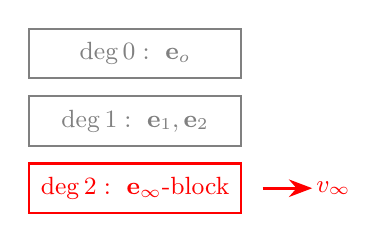
\begin{tikzpicture}[scale=0.9]
        \foreach \i/\lab/\c in {0/{$\deg 0:\ \eo$}/gray, 1/{$\deg 1:\ \mathbf{e}_1,\mathbf{e}_2$}/gray, 2/{$\deg 2:\ \einff\text{-block}$}/CCGAred}{
          \draw[\c, thick] (0,-\i*0.95) rectangle (3.0,-\i*0.95+0.7);
          \node[\c] at (1.5,-\i*0.95+0.35) {\small \lab};
        }
        \draw[CCGAred,-{Stealth}, very thick] (3.3,-1.55)--(4.0,-1.55);
        \node[CCGAred] at (4.3,-1.55) {\small $\vinf$};
      \end{tikzpicture}\\[0.2cm]
      {\small Only the deg-2 stratum survives the limit.}
  \end{columns}
\end{frame}

\begin{frame}[t]{Normalization of objects}
  Points and round objects are projective --- $\lambda p$ is the same object. Two ways to pin
  a representative:
  \vspace{0.25cm}

  \textbf{Finite objects --- fix the homogeneous coordinate.}
  Since $p\dotp\einff=-w$, divide by the weight:
  \[
    \boxed{\;\hat p = \frac{p}{-\,p\dotp\einff}\qquad\Longrightarrow\qquad \hat p\dotp\einff=-1\;}
  \]
  \vspace{0.05cm}

  \textbf{Scale-invariants --- no normalization needed.}
  \[
    \operatorname{sign}(s^2)\ \ (\text{reality}),\qquad\qquad
    r^2=\frac{s^2}{(s\dotp\einff)^2}\ \ (\text{invariant radius}) .
  \]
  \vspace{0.05cm}

  \textbf{Ideal objects} ($w=0$, $p\dotp\einff=0$). The $\einff$-scale degenerates --- no finite
  radius. Use the coordinate-free \alert{adaptive norm} $\hat A = A/\lVert A\rVert$, with
  $\lVert\cdot\rVert$ switching from the $\einff$-weight (finite) to the Euclidean direction
  norm (ideal).
\end{frame}

% ============================================================
% E. CONICS
% ============================================================
\section{Conics}

\begin{frame}[t]{IPNS: a grade-1 vector \emph{is} a general conic}
  For $q$ on the conic, $q\dotp s=0$ reproduces $Ax^2+By^2+Cxy+Dx+Ey+F=0$ with
  \[
    \boxed{\;
      s = -2A\,\eoi1 - 2B\,\eoi2 - C\,\eoi3 + D\,\mathbf{e}_1 + E\,\mathbf{e}_2
          - \tfrac{F}{2}(\einfi1+\einfi2)
    \;}
  \]
  \vspace{0.2cm}
  \begin{columns}[T]
    \column{0.5\textwidth}
      \textbf{Shape} $(A,B,C)$ lives on the \alert{origin} side
      $\eoi1,\eoi2,\eoi3$.
    \column{0.5\textwidth}
      \textbf{Size} $F$ lives on the \alert{infinity} side $\einff$;
      $(D,E)$ on $\mathbf{e}_1,\mathbf{e}_2$.
  \end{columns}
  \vspace{0.3cm}
  \textcolor{gray}{$q\dotp s$ never sees $\einfi3$ and sees $\einfi1,\einfi2$ only through their sum: $\einfi3$ and $\einfb$ are \alert{gauge-inert} (canonical form sets them $0$).}
\end{frame}

\begin{frame}[t]{OPNS: a grade-7 blade from five points}
  Five points fix a conic. The clean OPNS object wedges in the \alert{origin gauge}:
  \[
    \boxed{\;C = \Iod \wed p_1 \wed p_2 \wed p_3 \wed p_4 \wed p_5\;}
    \qquad\text{(grade 7)} .
  \]
  \vspace{0.2cm}
  Incidence is a single wedge, dual to the inner-product test:
  \[
    q\wed C = 0 \quad\Longleftrightarrow\quad q\dotp s = 0,
    \qquad s = C^\star \ (\text{grade }1) .
  \]
  \vspace{0.2cm}
  \begin{exampleblock}{Role of $\Iod$}
    Points only span a $6$-D subspace; the two directions they cannot reach are
    $\eob,\eoi3$, whose blade is $\Iod$. Wedging it supplies those directions and
    \alert{gauge-fixes the dual} to land on the clean grade-1 $s$.
  \end{exampleblock}
\end{frame}

\begin{frame}[t]{The wedge ladder}
  Each extra point raises the grade by one; the dual drops by one.
  \vspace{0.3cm}
  \begin{center}
  \renewcommand{\arraystretch}{1.25}
  \begin{tabular}{l c c l}
    object & OPNS & grade & dual grade\\
    \hline
    point      & $p$                                  & 1 & 1 (self)\\
    dipole     & $p_1\wed p_2$                        & 2 & 6\\
    tripole    & $p_1\wed p_2\wed p_3$                & 3 & 5\\
    quadpole   & $p_1\wed\cdots\wed p_4$              & 4 & 4\\
    \alert{pentapole} & $p_1\wed\cdots\wed p_5$       & 5 & 3 \;($-\tfrac12\,s\wed\Iinfd$)\\
    \alert{conic} & $\;\cdot\;\wed\Iod$               & 7 & 1 \;($=s$)\\
  \end{tabular}
  \end{center}
  \vspace{0.3cm}
  \begin{alertblock}{Key point}
    The \alert{pentapole already is} the conic as a point locus
    ($q\wed P_5=0\Leftrightarrow q$ on the conic). Wedging $\Iod$ adds \emph{no}
    geometry --- it only \alert{cleans the dual} from grade 3 to the grade-1 $s$.
  \end{alertblock}
\end{frame}

\begin{frame}[t]{Named conics: one vector $s$, six numbers}
  Every named conic is the same $s$ with a specific $(A,B,C,D,E,F)$:
  \vspace{0.2cm}
  \begin{center}
  \renewcommand{\arraystretch}{1.3}
  \small
  \begin{tabular}{l l l}
    conic & $(A,B,C,D,E,F)$ & type test\\
    \hline
    \alert{circle} $(c_x,c_y,r)$ & $(1,1,0,-2c_x,-2c_y,c_x^2{+}c_y^2{-}r^2)$ & $A{=}B,\,C{=}0,\ s^2{=}r^2$\\
    \alert{ellipse} $(a,b)$ & $(\tfrac1{a^2},\tfrac1{b^2},0,\dots)$ & $\Delta=C^2{-}4AB<0$\\
    \alert{hyperbola} $(a,b)$ & $(\tfrac1{a^2},-\tfrac1{b^2},0,\dots)$ & $\Delta>0$\\
    \alert{parabola} $y^2{=}4px$ & $(0,1,0,-4p,0,0)$ & $\Delta=0$\\
    \alert{tilted ellipse} $\theta$ & $C\neq0$ via $\eoi3$ & $\Delta<0$\\
    \alert{line} $n_xx{+}n_yy{+}d$ & $(0,0,0,n_x,n_y,d)$ & $A{=}B{=}C{=}0$ (no $\eo$)\\
    \alert{line pair} $\ell_1\ell_2$ & symmetric square of $\ell_1,\ell_2$ & $\det M_3=0$\\
  \end{tabular}
  \end{center}
  \vspace{0.2cm}
  \textcolor{gray}{A circle is $s=\pca-\tfrac{r^2}2\einff$ --- exactly the CGA form. A line is the most degenerate conic: it has \emph{no} origin part.}
\end{frame}

\begin{frame}[t]{Closed form of the dipole (point pair)}
  Parametrise by center $p$, unit direction $v$, signed radius $r$
  (endpoints $p\pm r v$). The quadratic point map collapses the wedge to
  \[
    \boxed{\;
      pp = p_1\wed p_2 = -2r\,\big(C + r^2\,\vinf\big)\wed W
    \;}
  \]
  \vspace{-0.2cm}
  \begin{columns}[T]
    \column{0.62\textwidth}
      \small
      \begin{align*}
        C       &= \eo + p_x\mathbf{e}_1 + p_y\mathbf{e}_2 + \cdots && (\text{center})\\
        W       &= v_x\mathbf{e}_1 + v_y\mathbf{e}_2 + \cdots && (\text{tangent }\mathrm dC[v])\\
        \vinf   &= \tfrac{v_x^2}2\einfi1+\tfrac{v_y^2}2\einfi2+v_xv_y\einfi3 && (\text{ideal pt of }v)
      \end{align*}
    \column{0.38\textwidth}
      \textbf{Reality} from $\mathrm{sign}(r^2)$:
      \[
        \begin{cases}
          r^2>0 & \text{two real pts}\\
          r^2=0 & \text{tangent / coincident}\\
          r^2<0 & \text{imaginary pair}
        \end{cases}
      \]
      \[ pp^2 = 4r^4 \]
  \end{columns}
\end{frame}

% ============================================================
% F. TYPE, FLATS, IDEAL ELEMENTS
% ============================================================
\begin{frame}[t]{Conic type = incidence with the line at infinity}
  Build a conic from \alert{3 points + an ideal-point pair} $B$
  (a line in the plane at infinity):
  \[
    C = p_1\wed p_2\wed p_3\wed B \wed \Iod .
  \]
  The type is how $B$'s line meets the conic-at-infinity (the Veronese cone):
  \vspace{0.2cm}
  \begin{center}
  \renewcommand{\arraystretch}{1.3}
  \begin{tabular}{l l l}
    $B$ (two ideal points) & line vs $\infty$-conic & type\\
    \hline
    $\vinf(v_1)\wed\vinf(v_2)$, real & secant & \alert{hyperbola} (dirs = asymptotes)\\
    one double direction & tangent & \alert{parabola}\\
    two imaginary directions & non-secant & \alert{ellipse}\\
    $\Iinfd$ (circular points) & non-secant & \alert{circle}\\
  \end{tabular}
  \end{center}
  \vspace{0.2cm}
  \textcolor{gray}{Reality here is \emph{not} $B^2$ (infinity is null, $B^2=0$): it is the secant / non-secant nature.}
\end{frame}

\begin{frame}[t]{Flats and ideal elements --- the join units}
  \begin{center}
  \renewcommand{\arraystretch}{1.35}
  \begin{tabular}{l l c}
    object & construction & grade\\
    \hline
    flat point & $p\wed\Iinf$ (pure position) & 4\\
    line (flat) & $p_1\wed p_2\wed\Iinf$ & 5\\
    plane (2-flat) & $p_1\wed p_2\wed p_3\wed\Iinf$ & 6\\
    line at infinity & $\Iinf$ & 3\\
    conic at infinity & $\Iod\wed\Iinf$ & 5\\
  \end{tabular}
  \end{center}
  \vspace{0.3cm}
  Composition: $\text{flat}\wed\text{flat}=0$ (repeated $\Iinf$),
  $\text{flat}\wed\text{ideal}=0$, $\text{flat}\wed\text{finite point}\to$ higher flat.
  \vspace{0.15cm}

  \textcolor{gray}{Flats are for \alert{joins}; the IPNS line (a degenerate conic) is for \alert{meets}.}
\end{frame}

% ============================================================
% G. CGA INSIDE CCGA
% ============================================================
\section{CGA lives inside CCGA}

\begin{frame}[t]{The circular points, and recovering CGA}
  \setlength{\columnsep}{16pt}
  \begin{columns}[T]
    \column{0.56\textwidth}
      The infinity gauge \alert{is} the pair of \alert{circular points} $I,J$:
      \[
        I=\vinf(1,i),\quad J=\vinf(1,-i),\qquad
        \boxed{\,I\wed J = -\,i\,\Iinfd\,}.
      \]
      \vspace{0.1cm}
      \emph{Every} circle passes through $I,J$; a general ellipse does not.

      \vspace{0.5cm}
      So wedging $\Iinfd$ = ``be round.'' It recovers the \alert{whole CGA round
      family inside CCGA} (each CGA object of grade $k$ lands at grade $k{+}2$):
      \[
        \text{round point } p\wed\Iinfd,\quad
        \text{circle } p_1\wed p_2\wed p_3\wed\Iinfd,\ \dots
      \]

    \column{0.44\textwidth}
      \centering
      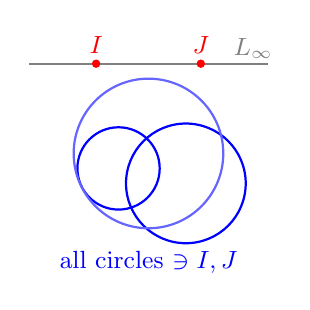
\begin{tikzpicture}[scale=0.95]
        \draw[gray, thick] (-1.6,1.4)--(1.6,1.4);
        \node[gray] at (1.4,1.6) {\small $L_\infty$};
        \fill[CCGAred] (-0.7,1.4) circle (1.6pt) node[above] {\small $I$};
        \fill[CCGAred] (0.7,1.4) circle (1.6pt) node[above] {\small $J$};
        \draw[CCGAblue, thick] (-0.4,0) circle (0.55);
        \draw[CCGAblue, thick] (0.5,-0.2) circle (0.8);
        \draw[CCGAblue!60, thick] (0.0,0.2) circle (1.0);
        \node[CCGAblue] at (0,-1.25) {\small all circles $\ni I,J$};
      \end{tikzpicture}
  \end{columns}
\end{frame}

% ============================================================
% H. INTERSECTIONS
% ============================================================
\section{Meet, intersections, pencils}

\begin{frame}[t]{Meet grade arithmetic}
  For blades in general position (pseudoscalar grade 8):
  \[
    \boxed{\;\operatorname{grade}(A\meet B)=\operatorname{grade}(A)+\operatorname{grade}(B)-8\;}
  \]
  Meaningful only when grades sum to $\ge 8$; grade $0$ is the \alert{incidence test}.
  \vspace{0.2cm}
  \begin{center}
  \renewcommand{\arraystretch}{1.2}
  \small
  \begin{tabular}{l c l}
    $A\meet B$ & grade & meaning\\
    \hline
    conic $\meet$ conic & $7{+}7{-}8=6$ & the 4 B\'ezout points\\
    conic $\meet$ line at $\infty$ & $7{+}3{-}8=2$ & the conic's 2 ideal points\\
    conic $\meet$ point & $7{+}1{-}8=0$ & incidence $q\meet C=0\Leftrightarrow q\in C$\\
  \end{tabular}
  \end{center}
  \vspace{0.2cm}
  \[
    C_1\meet C_2 \;\propto\; p_1\wed p_2\wed p_3\wed p_4\wed\Iod \;=\; Q\wed\Iod
    \quad(\text{grade }6).
  \]
\end{frame}

\begin{frame}[t]{B\'ezout reduction: the shared-factor principle}
  \setlength{\columnsep}{14pt}
  \begin{columns}[T]
    \column{0.58\textwidth}
      Recover the quadpole by contracting out the gauge:
      \[
        Q = (\einfi3\wed\einfb)\;\lrcorner\;(C_1\meet C_2).
      \]
      Its four points split by reality (sum $=4$, B\'ezout):
      \[
        \{\text{real}\}+\{\text{imaginary}\}+\{\text{ideal}\}=4 .
      \]
      \vspace{0.2cm}
      \[
        \boxed{\;\#\,\text{finite} = 4 - \#\,\text{forced common ideal points}\;}
      \]
      Two circles share $I,J$ $\Rightarrow$ \alert{2 finite} $+$ 2 ideal.
      \vspace{0.15cm}

      \textcolor{gray}{The fast dipole $\pm\sqrt{}$ shortcut is valid \emph{iff} both objects pass through $I,J$ (i.e. both are circles/lines); otherwise use the grade-4 quadpole route.}

    \column{0.42\textwidth}
      \centering
      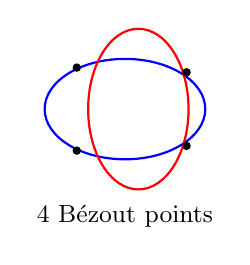
\begin{tikzpicture}[scale=0.85]
        \draw[CCGAblue, thick] (0,0) ellipse (1.2 and 0.75);
        \draw[CCGAred, thick] (0.2,0) ellipse (0.75 and 1.2);
        \foreach \p in {(0.92,0.55),(0.92,-0.55),(-0.72,0.62),(-0.72,-0.62)}{
          \fill[black] \p circle (1.8pt);}
        \node at (0,-1.6) {\small 4 B\'ezout points};
      \end{tikzpicture}
  \end{columns}
\end{frame}

\begin{frame}[t]{Pencils of conics}
  A \alert{pencil} is the linear family
  \[
    \Big\{\,\textstyle\sum_i \lambda_i\,C_i\,\Big\}
    \;=\; \text{dual of an } n\text{-blade over } (\eoi1,\eoi2,\eoi3,\mathbf{e}_1,\mathbf{e}_2,\einff).
  \]
  All members share the same intersection points.
  \vspace{0.3cm}
  \begin{itemize}\setlength\itemsep{0.3em}
    \item a single conic is a \alert{1-pencil}; $\Iod$ is the pencil of \emph{all} conics;
    \item add a conic: $P\meet C$ \quad(order $+1$);
    \item add a point: $P\wed p$ \quad(sub-pencil through $p$);
    \item with a right \alert{complement} $A^c$: remove a conic $P\wed C^c$, remove a point $P\meet p^c$.
  \end{itemize}
  \vspace{0.2cm}
  \textcolor{gray}{The complement-based calculus is the next slide's ``still to find.''}
\end{frame}

% ============================================================
% I. PROPERTIES
% ============================================================
\section{Properties, read off the algebra}

\begin{frame}[t]{Every conic invariant is an inner product of $s$}
  \[
    A=\tfrac12 s\dotp\einfi1,\quad B=\tfrac12 s\dotp\einfi2,\quad C=s\dotp\einfi3,\quad
    D=s\dotp\mathbf{e}_1,\quad E=s\dotp\mathbf{e}_2,\quad F=s\dotp\eo .
  \]
  Shape splits into an \alert{isotropic} part (size) and a \alert{deviatoric spin-2} part (tilt):
  \[
    \underbrace{A+B = s\dotp\einff}_{\text{trace / size}},\qquad
    \underbrace{(A-B,\;C)=(s\dotp\einfb,\;s\dotp\einfi3)}_{\text{anisotropy, angle }=2\theta} .
  \]
  \[
    \Delta_2 = AB-\tfrac{C^2}4,\qquad
    \lambda_\pm=\tfrac12 s\dotp\einff \pm \tfrac12\sqrt{(s\dotp\einfb)^2+(s\dotp\einfi3)^2},\qquad
    \theta=\tfrac12\operatorname{atan2}(s\dotp\einfi3,\,s\dotp\einfb).
  \]
  Center, semi-axes $a_i^2=-(\pca\dotp s)/\lambda_i$, eccentricity, foci, and asymptotic
  directions $\vinf\dotp s=0$ --- \alert{all GA}; only a final $\sqrt{}$ / $\operatorname{atan2}$ is scalar.
\end{frame}

% ============================================================
% J. VERSORS
% ============================================================
\section{Transformations}

\begin{frame}[t]{Versors: one sandwich for every object}
  $X\mapsto V X \widetilde V$ acts uniformly on points, pairs, lines, \emph{and} conics,
  preserving incidence.
  \vspace{0.2cm}
  \begin{center}
  \renewcommand{\arraystretch}{1.35}
  \small
  \begin{tabular}{l l}
    transform & versor\\
    \hline
    translation & $T=T_x T_y$ (products of $1-\tfrac\tau2\,\mathbf{e}_i\wed\einfi{j}$)\\
    \alert{rotation} $\alpha$ & $e^{\alpha E}e^{\alpha K}$, $\;K=\eob\wed\einfi3-\eoi3\wed\einfb$, $\;K^3=-4K$\\
    scaling $s$ & $\prod_{i=1}^3(\cosh u+\sinh u\,\eoi{i}\wed\einfi{i})$, $u=\tfrac12\ln s$\\
    reflection & $T(c)R(\theta)V_x\widetilde R(\theta)T(-c)$\\
    inversion / transversion & \alert{round family only} (M\"obius $\to$ quartic on general conics)\\
  \end{tabular}
  \end{center}
  \vspace{0.2cm}
  The rotor turns by $\alert{2\alpha}$ --- the \alert{Veronese symmetric-square} action --- which is
  exactly the spin-2 deviatoric pair $(\einfb,\einfi3)$ of the previous slide.
  Shear is non-conformal: \alert{no versor exists}.
\end{frame}

% ============================================================
% K. CLOSING
% ============================================================
\section{Synthesis and open problems}

\begin{frame}[t]{What is now pure geometric algebra}
  CCGA $\cong$ GAC (same metric, a basis change
  $\eo\!\leftrightarrow\!\bar n_+,\ \einff\!\leftrightarrow\! n_+,\ \eoi3\!\leftrightarrow\!\bar n_\times,\dots$).
  \vspace{0.4cm}
  \begin{exampleblock}{Structural operations expressed as GA products}
    \begin{itemize}\setlength\itemsep{0.25em}
      \item objects: points, conics (IPNS grade 1 $\leftrightarrow$ OPNS grade 7), flats, ideal elements;
      \item \alert{incidence}, \alert{type} (Veronese cone), reality;
      \item discriminants, \alert{center}, axes, eccentricity, foci, asymptotes --- inner products of $s$;
      \item intersections (meet), \alert{pencils};
      \item all rigid / conformal motions as versors.
    \end{itemize}
  \end{exampleblock}
\end{frame}

\begin{frame}[t]{Still to find --- the pure-GA gaps}
  Known GA formulas, not yet \alert{unified} into the framework:
  \vspace{0.3cm}
  \begin{itemize}\setlength\itemsep{0.5em}
    \item the right \alert{complement} $A^c$, defined by $A\wed A^c = I$ --- the operator the
          pencil and orthogonality calculus is built on;
    \item \alert{norm \& orthogonality}:
          $\;\lVert A\rVert=\sqrt{(A\wed A^c)^\star},\qquad A\perp B \iff A\wed B^c=0$;
    \item \alert{center / discriminants as a meet of three dual lines}:
          $\;\ell_1\meet\ell_2\meet\ell_3=\tfrac12\,\Delta_3\,\Iod\wed\Iinf$;
    \item the full complement-based \alert{pencil calculus}
          ($P\meet C,\ P\wed p,\ P\wed C^c,\ P\meet p^c$).
  \end{itemize}
  \vspace{0.3cm}
  \textcolor{gray}{These are structural and \emph{do} have GA forms --- the open work is to fold them into one consistent calculus (via $A^c$).}
\end{frame}

\begin{frame}[t]{Hard problems --- the irreducible scalar barrier}
  GA pushes every \alert{structural} step into blades. But \alert{extracting the actual
  points is not a GA product}:
  \vspace{0.25cm}
  \begin{itemize}\setlength\itemsep{0.35em}
    \item tripole $\to$ 3 points needs a \alert{cubic} (Cardano);
          quadpole / conic$\,\meet\,$conic $\to$ 4 points needs a \alert{quartic} (Ferrari).
          The dipole $\pm\sqrt{}$ has \emph{no} $n\ge3$ analogue.
  \end{itemize}
  \vspace{0.1cm}
  \begin{alertblock}{Why it is hard, not merely unimplemented}
    A blade is \alert{multilinear} (degree 1 in each point), yet the intersection points are
    the roots of a \alert{degree-$n$ polynomial}. Radical root-finding for degree $\ge3$
    (Abel--Ruffini) is not realizable by the bilinear GA products. GA gives the pencil
    reduction (resolvent cubic $+$ two $\pm\sqrt{}$ dipoles) cleanly; the final
    $\sqrt[3]{\ }/\sqrt{\ }$ stays an irreducible scalar step.
  \end{alertblock}
  \vspace{0.1cm}
  \textcolor{gray}{Still open too: a pure-GA \emph{line-pair factorization}. Objects are always GA multivectors --- and we can name exactly where the GA/numeric boundary sits.}
\end{frame}

%%%%%%%%%%%%%%%%%%%%%%%%%%%%%%%%%%%%%%%%%%%%%%%%%%%%%%%%%%%%%%%%%%%%
{\setbeamercolor{palette primary}{fg=black, bg=yellow}
  \begin{frame}[standout]
    Questions?
  \end{frame}
}
%%%%%%%%%%%%%%%%%%%%%%%%%%%%%%%%%%%%%%%%%%%%%%%%%%%%%%%%%%%%%%%%%%%%

\end{document}
